% DeepPEF_v5 teaching slide deck (Beamer). Compile with: pdflatex DeepPEF_v5_Slides.tex
% Figures generated by make_figures.py must exist in ./figures/.
\documentclass[aspectratio=169]{beamer}
\usetheme{metropolis}
\usepackage{graphicx}
\usepackage{booktabs}
\usepackage{xcolor}
\definecolor{acc}{HTML}{DD8452}
\definecolor{blue1}{HTML}{4C72B0}
\setbeamercolor{frametitle}{bg=blue1}
\graphicspath{{figures/}}

\title{DeepPEF\,v5 — The Six Levers (A–F)}
\subtitle{Physics-grounded, flag-gated, ablatable. Default = OFF = baseline.}
\date{}
\author{Teaching deck}

\begin{document}

\maketitle

\begin{frame}{The core idea}
  \centering
  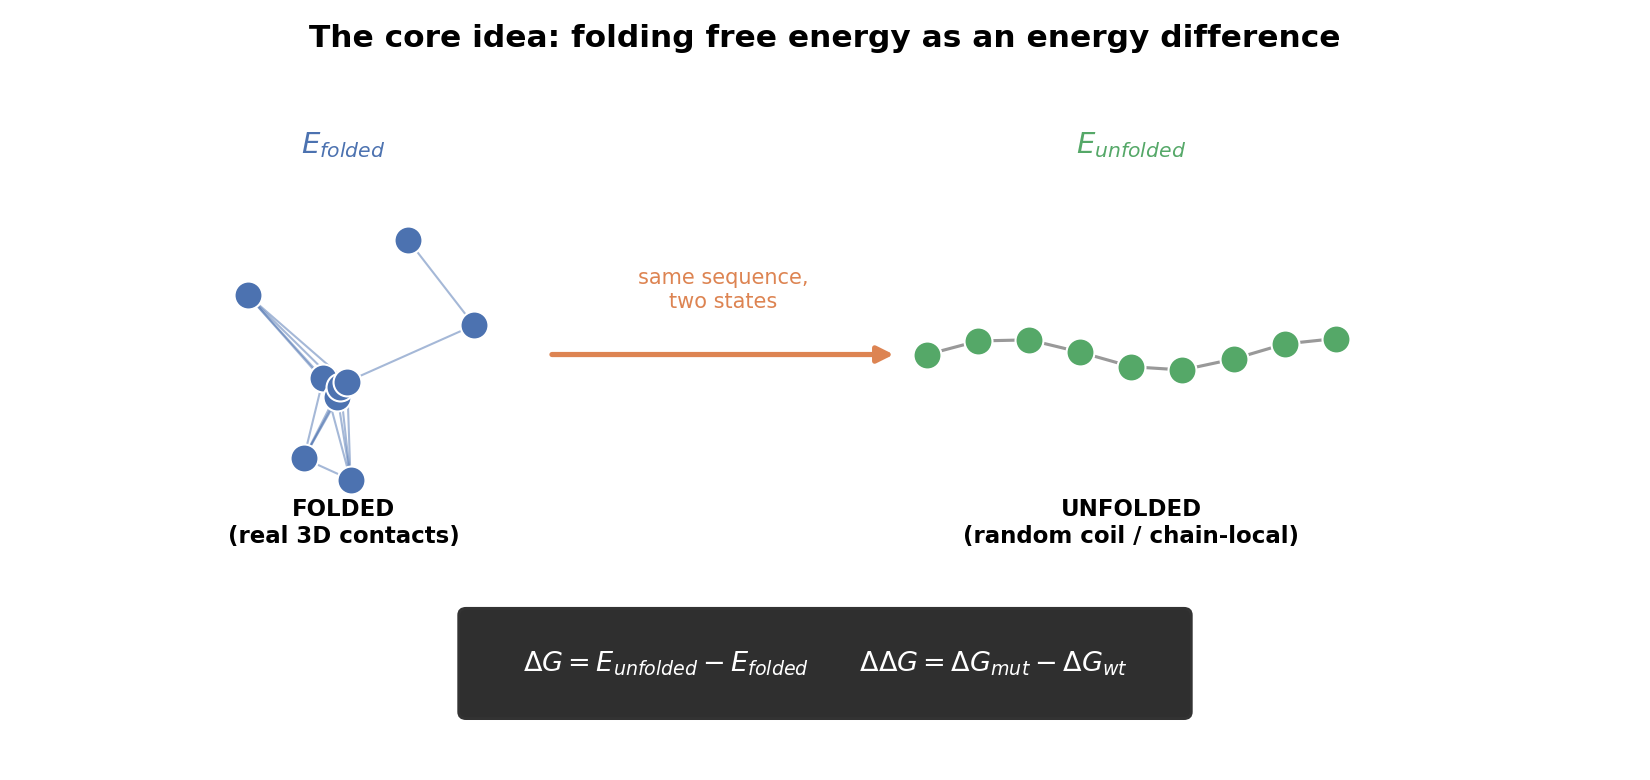
\includegraphics[width=.92\linewidth]{fig1_dg_concept.png}
  \vspace{0.3em}
  \footnotesize A folded graph (real 3D contacts) vs an unfolded reference (chain-local).
  $\Delta G = E_{unfolded}-E_{folded}$;\; $\Delta\Delta G = \Delta G_{mut}-\Delta G_{wt}$.
\end{frame}

\begin{frame}{The dimension contract}
  \centering
  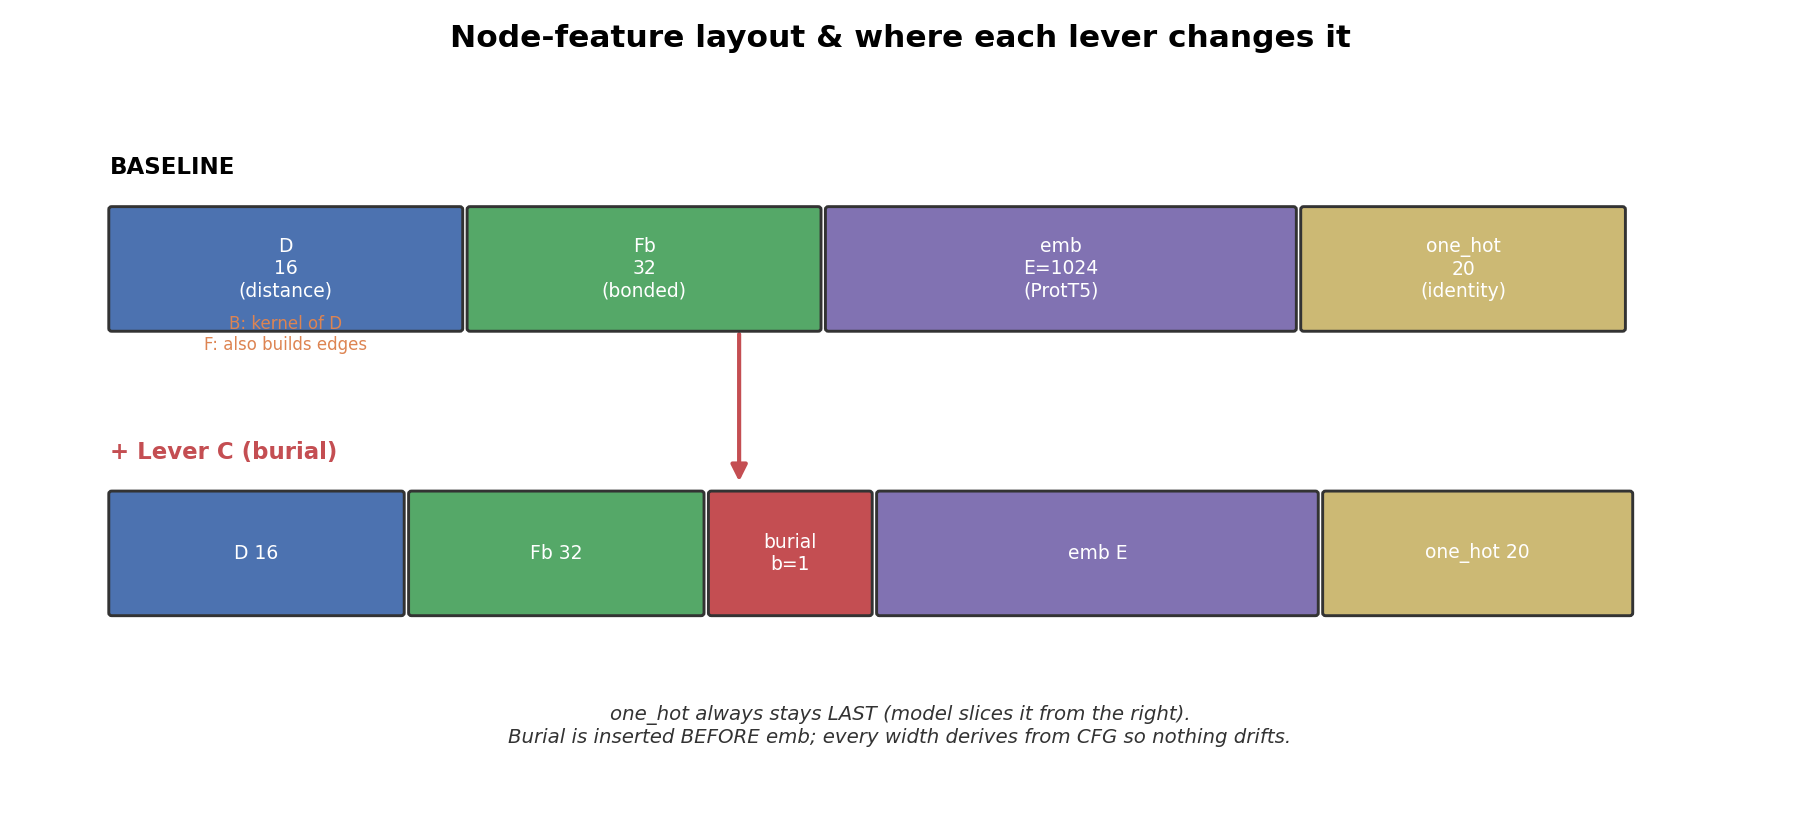
\includegraphics[width=.72\linewidth]{fig2_node_layout.png}
  \vspace{0.2em}
  \footnotesize Every width derives from ONE \texttt{CFG}. Builder and model read the same
  numbers, so a lever's default reproduces the baseline tensors bit-for-bit.
\end{frame}

\begin{frame}{The two-tower architecture}
  \centering
  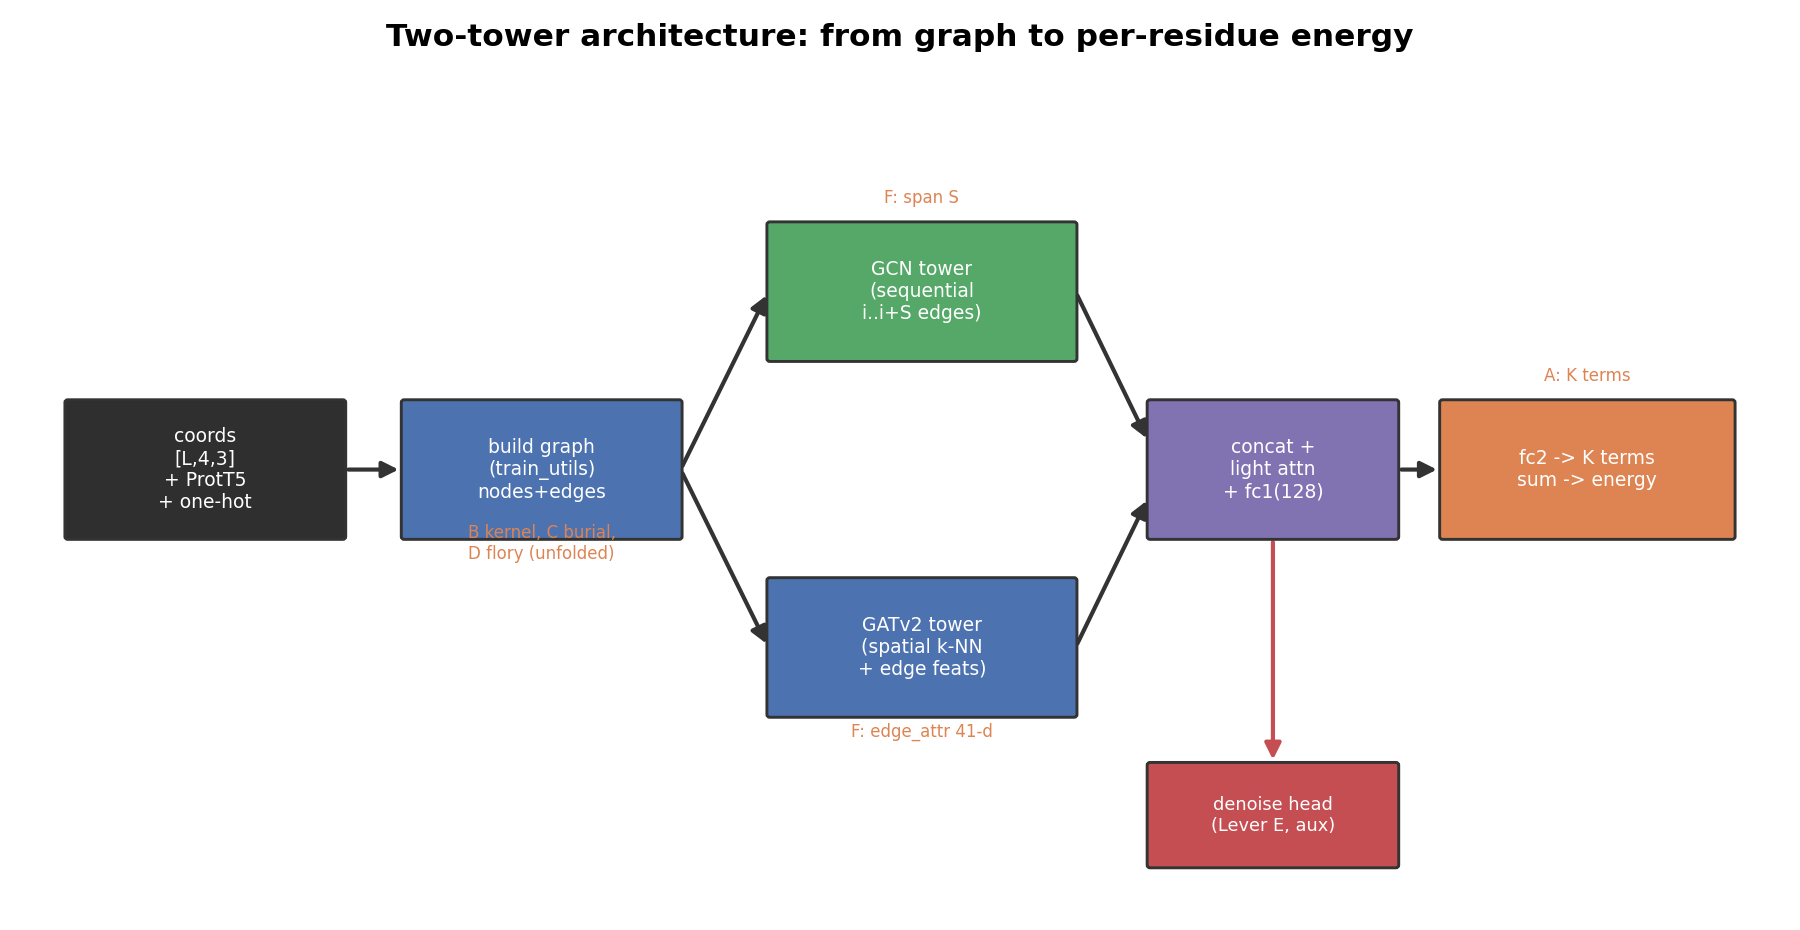
\includegraphics[width=.95\linewidth]{fig3_architecture.png}
\end{frame}

\begin{frame}{The six levers at a glance}
  \centering
  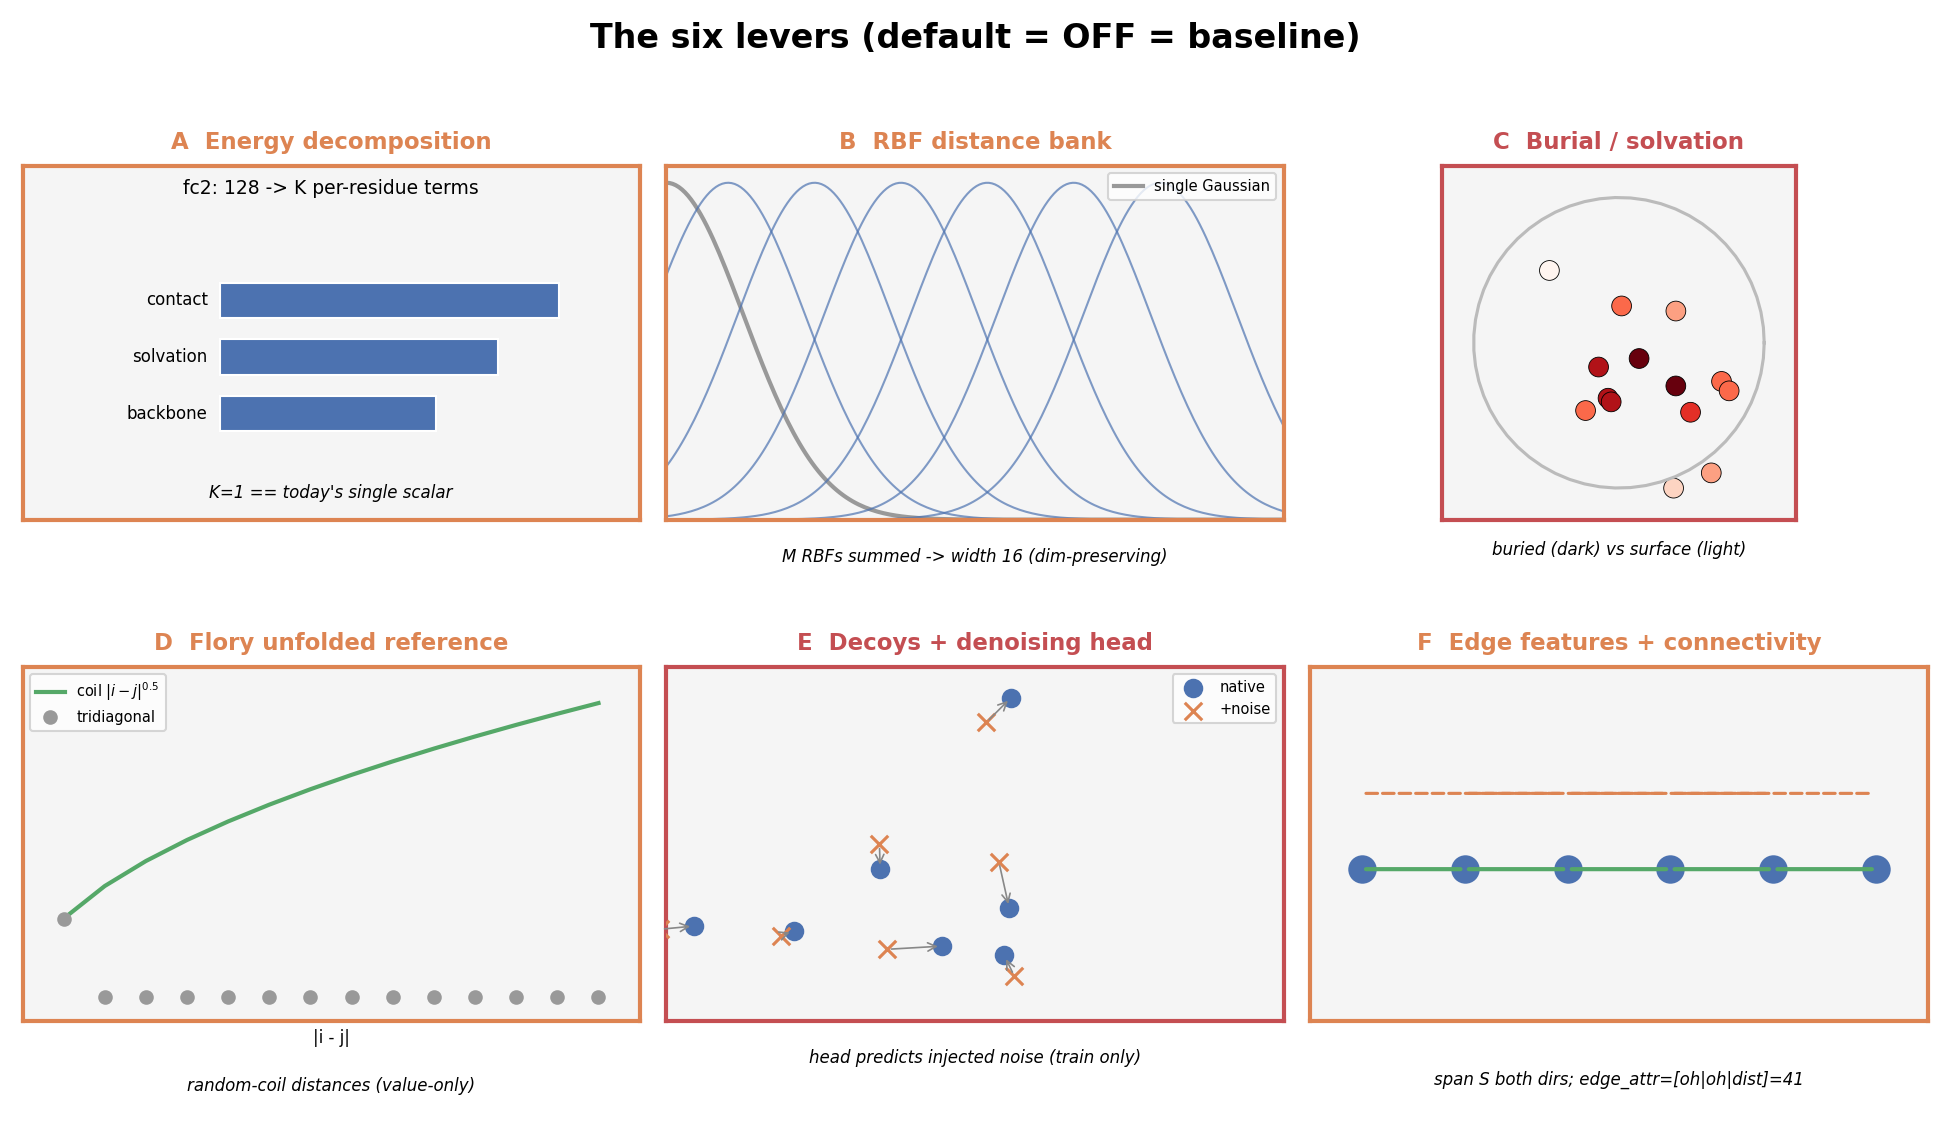
\includegraphics[width=.95\linewidth]{fig4_levers_grid.png}
\end{frame}

\begin{frame}{What each lever does}
  \scriptsize
  \begin{tabular}{@{}llp{6.8cm}@{}}
    \toprule
    Lever & Flag & Effect (default reproduces baseline) \\
    \midrule
    A & \texttt{--energy\_terms K} & \texttt{fc2} emits K per-residue energy terms; K=1 = scalar. \\
    B & \texttt{--rbf\_centers M} & M RBFs summed back to width 16 (dimension-preserving). \\
    C & \texttt{--use\_burial} & CB neighbor-density scalar inserted before emb. \\
    D & \texttt{--flory\_unfolded} & random-coil unfolded reference $d\sim|i-j|^{\nu}$ (value-only). \\
    E & \texttt{--denoise\_weight w} & aux head predicts injected coord noise (train only). \\
    F & \texttt{--gcn\_span S}, \texttt{--use\_edge\_features} & span-S GCN edges + 41-d GAT edge features. \\
    \bottomrule
  \end{tabular}
\end{frame}

\begin{frame}{Why the levers compose}
  \centering
  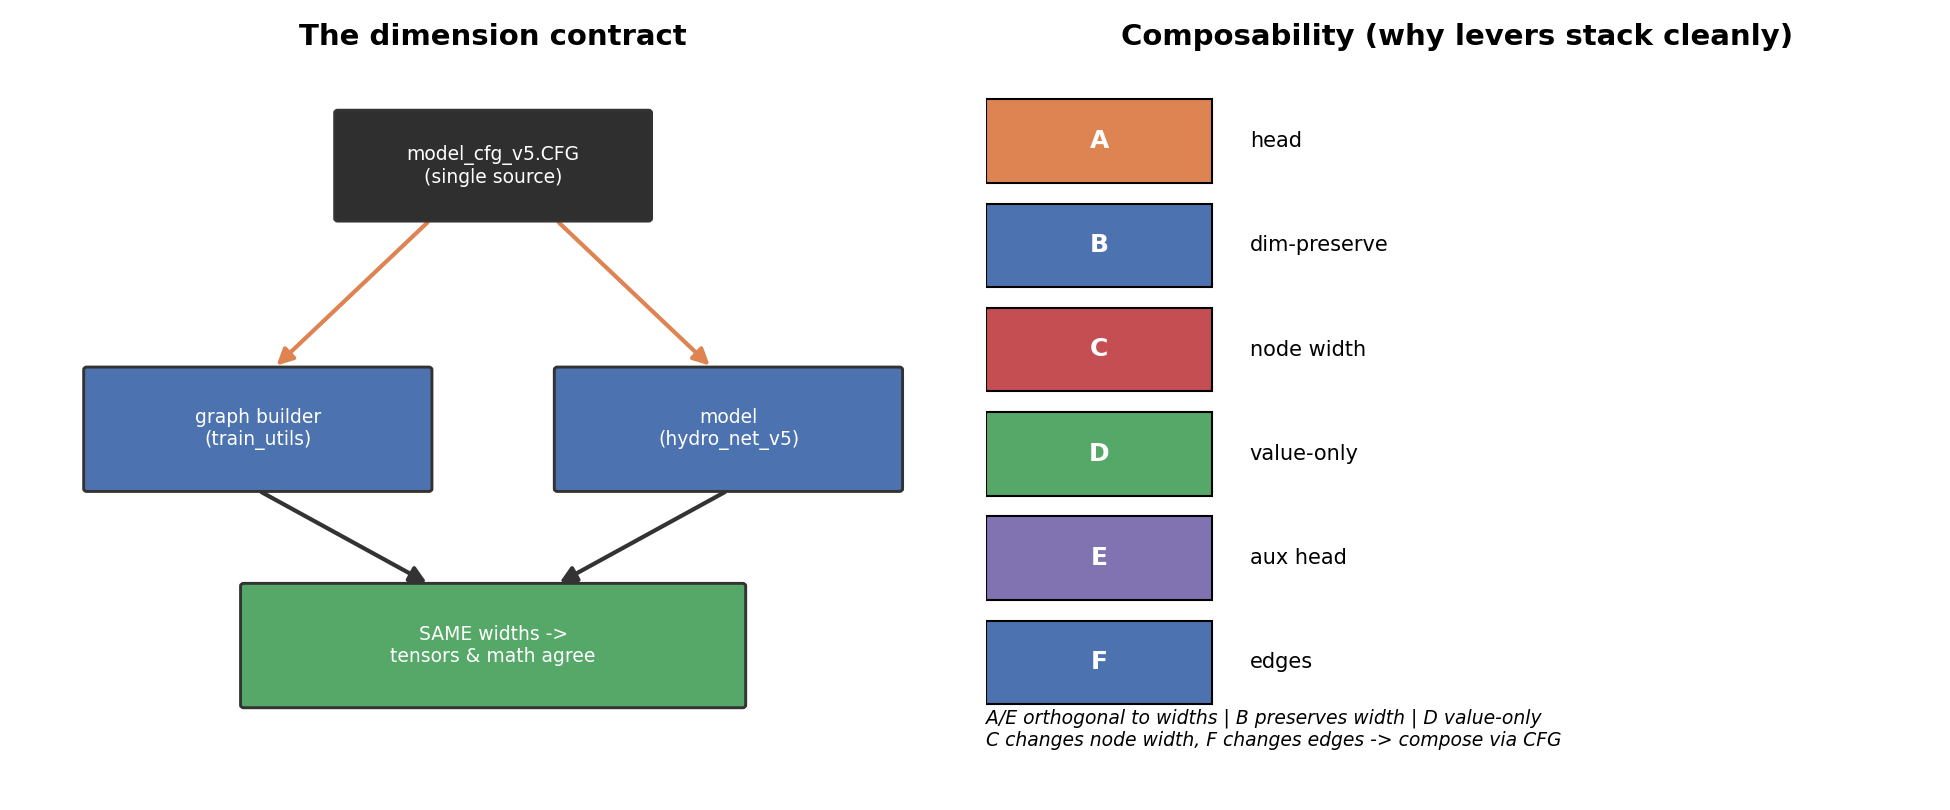
\includegraphics[width=.95\linewidth]{fig5_flow_compose.png}
\end{frame}

\begin{frame}{Verification}
  \begin{itemize}
    \item CPU smoke test runs baseline \textbf{and each lever} on synthetic data — no GPU, no real data.
    \item Baseline regression: default flags $\Rightarrow$ no denoise/edge params, \texttt{fc2}=(1,128),
          \texttt{burial\_dim}=0, \texttt{gcn\_span}=1.
    \item Fail-fast checks name the offending lever on any bad config or width mismatch.
    \item GPU ablation ladder measures PCC one lever at a time.
  \end{itemize}
  \vspace{1em}
  \centering \texttt{python DeepPEF\_v5/tests/smoke\_test.py}\; $\to$\; all configs PASS.
\end{frame}

\begin{frame}{Evaluation metrics}
  \small
  \begin{itemize}
    \item \textbf{PCC} (primary): $r=\mathrm{cov}(p,y)/(\sigma_p\sigma_y)$ — linear trend,
          shift/scale-invariant. Historical best \textbf{$\approx$0.5259}.
    \item \textbf{Spearman $\rho$}: Pearson on ranks — monotonic ordering, outlier-robust.
    \item \textbf{RMSE} $=\sqrt{\mathrm{mean}((p-y)^2)}$ — absolute error (diagnostic; energy is
          in relative units, not calibrated kcal/mol).
  \end{itemize}
  \vspace{0.5em}
  \footnotesize Correlation grades the \emph{pattern} (what matters for ranking variants); RMSE
  grades \emph{calibration}. We report all three.
\end{frame}

\begin{frame}{Loss functions}
  \small
  \[ \texttt{loss} = \texttt{primary} + \texttt{reg} + \texttt{energy\_reg} + \texttt{rank} +
     \texttt{corr}\;(+\,\texttt{denoise}) \]
  \begin{itemize}
    \item \textbf{Huber} ($\delta{=}1$): MSE near zero, L1 far out — robust to noisy labels.
    \item \textbf{Margin ranking}: $\max(0,-s\cdot\Delta p+\text{margin})$ — optimizes pairwise order.
    \item \textbf{Energy reg} $0.001\lVert E\rVert^2$ — anchors the extensive energy scale.
    \item \textbf{Pearson loss} $1-r$; \textbf{CCC loss} $1-\mathrm{CCC}$ (also penalizes shift + scale).
    \item \textbf{Denoise MSE} (Lever E) — consistency under structural noise.
  \end{itemize}
\end{frame}

\begin{frame}{Dataset biology}
  \small
  \begin{itemize}
    \item \textbf{Tsuboyama et al.\ 2023} mega-scale stability dataset.
    \item \textbf{K50 cDNA-display proteolysis}: folded proteins resist protease; K50 = cleavage
          midpoint $\to$ folding free energy $dG$. Higher K50 = more stable.
    \item \textbf{Clamp $dG\in[-1,5]$ kcal/mol} (\texttt{--dg\_ml}) — the assay's dynamic range.
    \item \textbf{Single mutations + PNAS curation} (\texttt{--one\_mut}) — quality $>$ quantity;
          unfiltered data \emph{hurt} performance.
    \item \textbf{ThermoMPNN} proteins + homologs held out — prevents test leakage.
  \end{itemize}
\end{frame}

\begin{frame}{EBM pretraining \& the physics bet}
  \small
  \begin{itemize}
    \item \textbf{Native = energy minimum}: shape the landscape so the native fold is lowest.
    \item \textbf{InfoNCE / Boltzmann}: $L = E_{native}/\tau + \log\sum_k e^{-E_k/\tau}$
          (negatives: decoy seq/structure, unfolded, cyclic perms).
    \item \textbf{DSM}: teach $\nabla E$ to point back to native under noise
          ($v\cdot\nabla E \approx v\cdot(-\text{noise}/\sigma^2)$) $\to$ Lever E at fine-tuning.
  \end{itemize}
  \vspace{0.4em}
  \footnotesize Physics bet: fold$-$unfold difference + extensive (summed) energy + Flory reference
  shrink the hypothesis space to physically plausible functions — for data efficiency,
  interpretability, and generalization.
\end{frame}

\begin{frame}{Limitations \& scope}
  \small
  \begin{itemize}
    \item No inverse-folding pretraining in baseline (largest known lever; the gap to ThermoMPNN).
    \item Fixed WT structure per protein — no mutation-induced local relaxation.
    \item Extensive energy confounds length unless \texttt{length\_norm} is on.
    \item Relative-unit energy — RMSE is a diagnostic, not calibrated kcal/mol.
    \item Glycine virtual-CB caveat; ESM-IF 1536-d alignment relies on the CFG contract.
  \end{itemize}
\end{frame}

\end{document}
